\section{Kiến trúc mô hình}
\label{sec:model}

\subsection{Đầu vào của mô hình}
\label{subsec:model_input}

Mô hình được thiết kế để xử lý dữ liệu giao thông theo vùng, trong đó mỗi mẫu đầu vào bao gồm
chuỗi quan sát giao thông trong một cửa sổ thời gian, cùng với thông tin ngữ cảnh không gian
và thời gian tương ứng. Cụ thể, đầu vào của mô hình bao gồm ba thành phần chính:

\begin{itemize}
    \item \textbf{Chuỗi giao thông theo vùng:} lịch sử tốc độ giao thông của các tuyến đường
    trong cùng một vùng giao thông chức năng.
    \item \textbf{Thông tin thời gian:} bao gồm thời điểm trong ngày và ngày trong tuần,
    được mã hóa thông qua Temporal Encoding nhằm phản ánh tính chu kỳ của giao thông đô thị.
    \item \textbf{Thông tin không gian:} biểu diễn vị trí cấu trúc của các tuyến đường trong vùng
    thông qua Laplacian Positional Encoding dựa trên phổ đồ thị.
\end{itemize}

Ba thành phần này được kết hợp tại tầng embedding đầu vào và cung cấp cho Transformer encoder
một biểu diễn thống nhất, trong đó mỗi token đồng thời mang thông tin giao thông, vị trí không
gian và ngữ cảnh thời gian.

\subsection{Attention score bias trong Transformer}
\label{subsec:attention_bias}

Khác với Transformer tiêu chuẩn, trong đó trọng số attention chỉ phụ thuộc vào độ tương đồng
giữa truy vấn (query) và khóa (key), mô hình của nhóm cho phép tích hợp thêm một
\textit{attention score bias} bằng cách cộng một thành phần điều chỉnh vào ma trận điểm
attention trước khi áp dụng hàm softmax. Cụ thể, với một head attention, điểm attention giữa
hai token $i$ và $j$ được tính như sau:
\begin{equation}
\alpha_{i,j}
=
\frac{
\mathbf{q}_i^\top \mathbf{k}_j
}{
\sqrt{d_k}
}
+
\gamma \, B_{i,j},
\end{equation}
trong đó $\mathbf{q}_i$ và $\mathbf{k}_j$ lần lượt là vector truy vấn và khóa tương ứng,
$d_k$ là kích thước không gian khóa, $B_{i,j}$ là attention bias phản ánh mối quan hệ chức
năng giữa hai token, và $\gamma$ là một hệ số vô hướng được học trong quá trình huấn luyện.

Sau đó, trọng số attention được chuẩn hóa theo softmax:
\begin{equation}
\text{Attn}_{i,j}
=
\frac{
\exp(\alpha_{i,j})
}{
\sum_{j'} \exp(\alpha_{i,j'})
}.
\end{equation}

Attention bias $B_{i,j}$ được xây dựng bên ngoài mô hình Transformer và đóng vai trò mã hóa
thông tin bổ sung về quan hệ giữa các tuyến đường trong cùng một vùng giao thông, chẳng hạn
như mối tương quan giao thông có độ trễ hoặc mối liên hệ không gian--cấu trúc trong mạng lưới.
Việc đưa bias vào dưới dạng một thành phần cộng cho phép mô hình điều chỉnh điểm attention
mà không làm thay đổi cấu trúc cơ bản của cơ chế self-attention.

Khác với các Transformer đồ thị như Graphormer, trong đó bias cấu trúc thường được thiết kế
cố định và phụ thuộc vào khoảng cách đồ thị toàn cục, attention bias trong mô hình của chúng
tôi mang tính linh hoạt theo từng vùng giao thông và từng thời điểm. Hơn nữa, hệ số $\gamma$
được học cho phép mô hình tự động cân bằng giữa thông tin cấu trúc được mã hóa trong bias và
độ tương đồng ngữ nghĩa thuần túy giữa các token.

Trong quá trình thực nghiệm, nhóm đã từng làm mô hình không sử dụng attention score
bias trong cùng một thiết lập huấn luyện. Kết quả cho thấy, mô hình không có attention bias kém hiệu quả hơn. Mô hình tích hợp attention bias giúp cải thiện độ ổn định của quá trình huấn luyện và mang lại hiệu năng dự báo tốt hơn so với
Transformer tiêu chuẩn không có bias. Điều này cho thấy rằng việc đưa thông tin quan hệ chức
năng trực tiếp vào điểm attention là một cơ chế hiệu quả để tăng cường khả năng mô hình hóa
các tương tác không gian--thời gian trong bài toán giao thông đô thị.


\subsection{Transformer encoder-only theo phong cách BERT}
\label{subsec:encoder_only}

\begin{figure}[H]
    \centering
    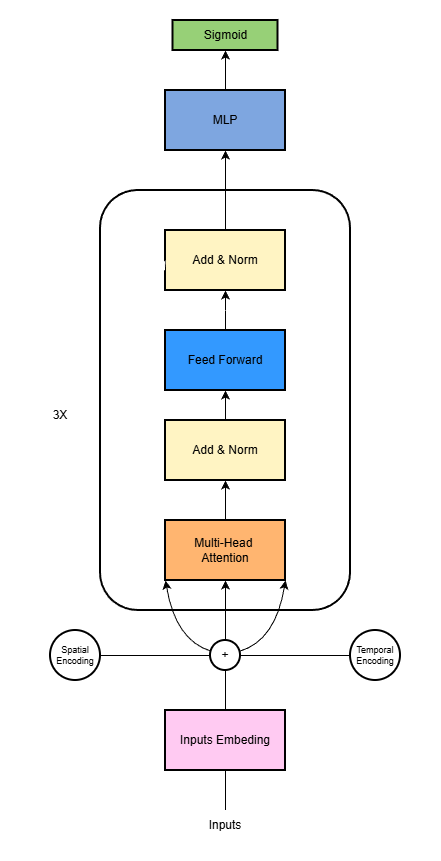
\includegraphics[width=0.5\textwidth]{Contents/MKhang/BERT.drawio.png}
    \caption{Kiến trúc mô hình Transformer encoder-only với Spatial và Temporal Encoding}
    \label{fig:model}
\end{figure}


Sau khi kết hợp các embedding đầu vào, dữ liệu được đưa vào một Transformer encoder-only
theo phong cách BERT. Kiến trúc này bao gồm nhiều lớp encoder xếp chồng, mỗi lớp có cùng
cấu trúc chuẩn gồm self-attention đa đầu và mạng feed-forward theo vị trí.



Mỗi lớp Transformer encoder trong mô hình bao gồm hai khối chính. Khối thứ nhất là
\textit{multi-head self-attention}, cho phép mỗi token trong vùng giao thông tương tác trực
tiếp với tất cả các token khác trong cùng cửa sổ thời gian, nhờ đó mô hình có thể học được
các quan hệ không gian--thời gian mang tính toàn cục.

Khối thứ hai là \textit{feed-forward network} (FFN), bao gồm hai lớp tuyến tính với hàm kích
hoạt phi tuyến ở giữa. FFN được áp dụng độc lập cho từng token và đóng vai trò tăng khả năng
biểu diễn phi tuyến của mô hình sau bước attention.

Trong mỗi lớp encoder, chuẩn hóa lớp (Layer Normalization) được áp dụng trước mỗi khối
self-attention và FFN, theo thiết kế \textit{pre-norm}. Thiết kế này giúp ổn định quá trình
huấn luyện, đặc biệt khi sử dụng nhiều lớp encoder. Các kết nối dư (residual connections)
được sử dụng xuyên suốt để bảo toàn thông tin và hỗ trợ lan truyền gradient.

Để giảm hiện tượng overfitting, dropout được áp dụng tại các đầu ra của self-attention và
bên trong mạng feed-forward. Việc sử dụng dropout ở nhiều vị trí giúp mô hình tổng quát
tốt hơn khi huấn luyện trên dữ liệu giao thông có tính nhiễu và biến động cao.

\subsection{Lớp dự đoán MLP}
\label{subsec:mlp_head}

Sau khi đi qua các lớp Transformer encoder, mô hình sử dụng biểu diễn tại thời điểm cuối
của cửa sổ thời gian để thực hiện dự đoán. Đối với mỗi tuyến đường trong vùng, embedding
tương ứng được đưa qua một lớp MLP dùng chung tham số giữa các tuyến.

Lớp MLP này bao gồm một tầng ẩn với hàm kích hoạt phi tuyến, tiếp theo là dropout để
giảm overfitting, và một tầng tuyến tính cuối cùng sinh ra một logit cho mỗi tuyến.
Thiết kế MLP nông giúp giữ cho tầng dự đoán đơn giản, trong khi phần lớn năng lực mô hình
được tập trung vào việc học biểu diễn không gian--thời gian thông qua Transformer encoder.

Kiến trúc dự đoán này phù hợp với giả định rằng các tuyến đường trong cùng một vùng giao
thông chia sẻ các quy luật động học tương tự, đồng thời cho phép mô hình tổng quát hóa tốt
sang các vùng giao thông khác nhau.
